\begin{frame}{Capitulando}

    \begin{columns}
        \column{0.5\textwidth}
            \hspace{0.75cm}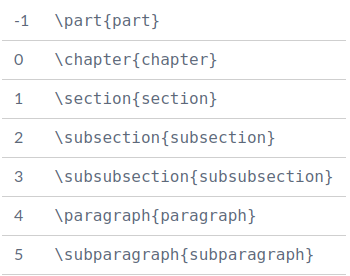
\includegraphics[width=0.75\textwidth]{images/sections.png}

        \column{0.5\textwidth}
            \begin{itemize}
                \item En artículos, lo más alto es la sección
                \item En \textit{report} y \textit{book}, lo más alto es \texttt{part} y \texttt{chapter} 
            \end{itemize}
    \end{columns}
    
    \vspace{0.5cm}
    \pause
    
    \begin{block}{}
    El comando \texttt{\textbackslash tableofcontents\{\}} crea el índice del documento (se puede poner en su propia página).\\
    \texttt{\textbackslash listoffigures\{\}} y \texttt{\textbackslash listoftables\{\}} hacen lo mismo con las figuras y tablas del documento\ldots{}
    \end{block}
    
\end{frame}